\documentclass{beamer}

% to include graphics
\usepackage{graphicx}

% to include hyperlinks
\usepackage{hyperref}

% divide slides into columns
\usepackage{multicol}


\usetheme{Copenhagen}
\usecolortheme{beaver}

\title{Cluster Progress}
\date{\today}

\begin{document}

%----------BEGIN TITLE----------

\begin{frame}
  \maketitle
\end{frame}

%-----------END TITLE-----------

%----------BEGIN NODES----------

\begin{frame}

  \frametitle{Incorporating the Nodes}
  
  \begin{multicols}{2}

    \begin{itemize}
    \item The boot order of nearly all the nodes has been modified.
      \begin{itemize}
      \item {\tt compute-0-9} and {\tt compute-1-9} are having issues
      \end{itemize}
    \item The nodes have been brought into the cluster via {\tt
        insert-ethers}!
    \item NOTE: They cannot all be turned on at the same time due to UPS
      bandwidth issues.
    \end{itemize}
    
    \columnbreak
    
    \begin{figure}[H]
      \begin{center}
        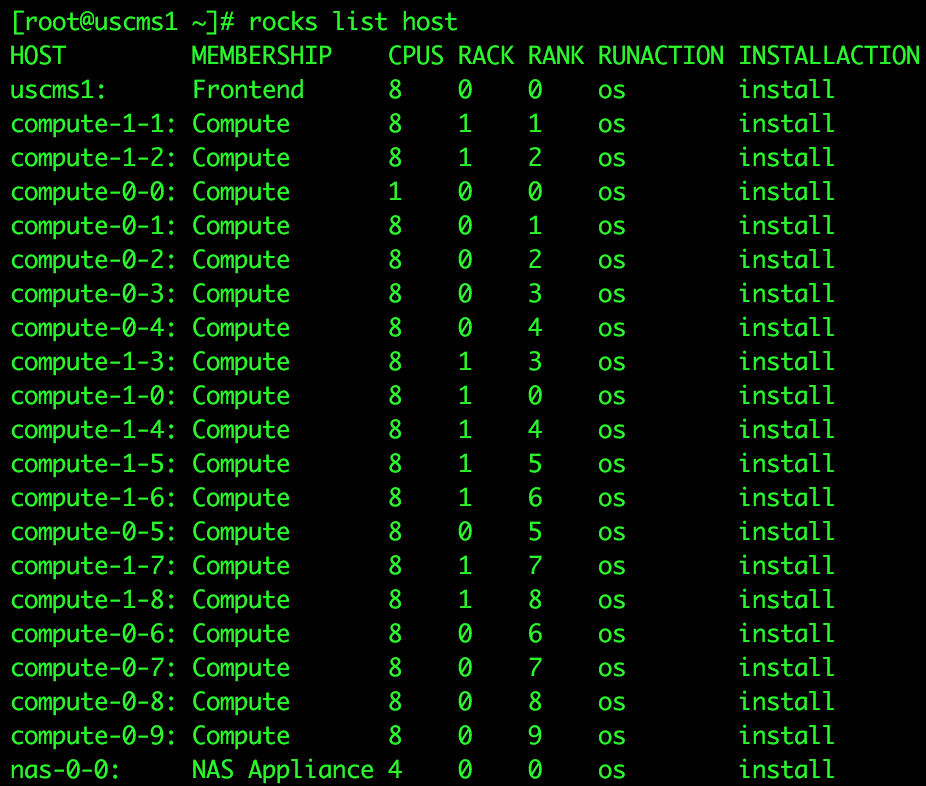
\includegraphics[scale=0.35]{CEHostList.png}
      \end{center}
      \caption{The list of all the hosts known to the CE. {\tt compute-1-9} is
        absent due to PXE boot issues, and NAS-0 is included, although it lacks
        the latest version of ROCKS.}
    \end{figure}
  
  \end{multicols}
  
\end{frame}

%-----------END NODES-----------

%----------BEGIN NAS-0----------

\begin{frame}
  
  \frametitle{Incorporating NAS-0}

  \begin{itemize}
    \item NAS-0 must be brought into the cluster in a similar manner to that of
      the nodes.
    \item It's boot order was changed for network boot, it obtained the
      kickstart file, and {\tt insert-ethers} recognized it.
    \item Installing the OS on the proper drive is proving troublesome.
      \begin{itemize}
        \item We only see the 14 drives part of the ZFS array, not the two
          drives in RAID-1 allocated for storing the OS. 
      \end{itemize}
  \end{itemize}

\end{frame}

%-----------END NAS-0-----------


\end{document}
